% Options for packages loaded elsewhere
\PassOptionsToPackage{unicode}{hyperref}
\PassOptionsToPackage{hyphens}{url}
%
\documentclass[
]{article}
\usepackage{lmodern}
\usepackage{amssymb,amsmath}
\usepackage{ifxetex,ifluatex}
\ifnum 0\ifxetex 1\fi\ifluatex 1\fi=0 % if pdftex
  \usepackage[T1]{fontenc}
  \usepackage[utf8]{inputenc}
  \usepackage{textcomp} % provide euro and other symbols
\else % if luatex or xetex
  \usepackage{unicode-math}
  \defaultfontfeatures{Scale=MatchLowercase}
  \defaultfontfeatures[\rmfamily]{Ligatures=TeX,Scale=1}
\fi
% Use upquote if available, for straight quotes in verbatim environments
\IfFileExists{upquote.sty}{\usepackage{upquote}}{}
\IfFileExists{microtype.sty}{% use microtype if available
  \usepackage[]{microtype}
  \UseMicrotypeSet[protrusion]{basicmath} % disable protrusion for tt fonts
}{}
\makeatletter
\@ifundefined{KOMAClassName}{% if non-KOMA class
  \IfFileExists{parskip.sty}{%
    \usepackage{parskip}
  }{% else
    \setlength{\parindent}{0pt}
    \setlength{\parskip}{6pt plus 2pt minus 1pt}}
}{% if KOMA class
  \KOMAoptions{parskip=half}}
\makeatother
\usepackage{xcolor}
\IfFileExists{xurl.sty}{\usepackage{xurl}}{} % add URL line breaks if available
\IfFileExists{bookmark.sty}{\usepackage{bookmark}}{\usepackage{hyperref}}
\hypersetup{
  pdftitle={Measuring the Statistical Performance of Countries: An Overview of the SPI Index},
  pdfauthor={SPI Team},
  hidelinks,
  pdfcreator={LaTeX via pandoc}}
\urlstyle{same} % disable monospaced font for URLs
\usepackage[margin=1in]{geometry}
\usepackage{graphicx}
\makeatletter
\def\maxwidth{\ifdim\Gin@nat@width>\linewidth\linewidth\else\Gin@nat@width\fi}
\def\maxheight{\ifdim\Gin@nat@height>\textheight\textheight\else\Gin@nat@height\fi}
\makeatother
% Scale images if necessary, so that they will not overflow the page
% margins by default, and it is still possible to overwrite the defaults
% using explicit options in \includegraphics[width, height, ...]{}
\setkeys{Gin}{width=\maxwidth,height=\maxheight,keepaspectratio}
% Set default figure placement to htbp
\makeatletter
\def\fps@figure{htbp}
\makeatother
\setlength{\emergencystretch}{3em} % prevent overfull lines
\providecommand{\tightlist}{%
  \setlength{\itemsep}{0pt}\setlength{\parskip}{0pt}}
\setcounter{secnumdepth}{-\maxdimen} % remove section numbering
\ifluatex
  \usepackage{selnolig}  % disable illegal ligatures
\fi

\title{Measuring the Statistical Performance of Countries: An Overview
of the SPI Index}
\author{SPI Team}
\date{2020-09-18}

\begin{document}
\maketitle
\begin{abstract}
Recognizing the new challenges for national statistical systems in
monitoring the Sustainable Development Goals (SDGs), the World Bank is
developing a new, improved Statistical Performance Indicators (SPI) to
monitor progress of the statistical performance of countries. This will
replace the Statistical Capacity Index (SCI) the World Bank has
regularly published since 2004. This short note briefly discusses the
motivation behind the new SPI, describes some of its major features, and
discusses a new index based on the indicators.
\end{abstract}

\hypertarget{motivation}{%
\section{Motivation}\label{motivation}}

The primary purpose of the statistical system is to help users of
statistics make better decisions or to hold those decision makers
accountable. In the words of Principle 1 of the Fundamental Principles
of Official Statistics, the statistics must ``meet the test of practical
utility'', serving ``the Government, the economy and the public with
data about the economic, demographic, social and environmental
situation.'' The national statistical system, or NSS, plays a crucial
role in modern economies. It provides stakeholders, ranging from policy
makers to stock market analysts and the general public, with the latest
data on the country's socio-economic developments. At the international
level, monitoring progress on global undertakings such as the recently
established Sustainable Development Goals (SDGs) requires high-quality
data that must be produced consistently across different national
statistical systems. Assessing and improving the capacity of a country's
NSS has long been a part of the global agenda. Since the early 2000s, a
few capacity assessment tools have been developed to identify the
weaknesses and strengths of national statistical systems by other
organizations including PARIS21, the Food and Agriculture Organization
of the United Nations (FAO), the United Nations Economic Commission for
Europe (UNECE), the United Nations Economic Commission for Africa
(UNECA), and the U.S. Census Bureau.

The World Bank's Statistical Capacity Index (SCI) is one such tool that
has been widely employed. Several international and national agencies
have adopted the SCI for measuring progress in statistical capacity
building and related investments. The World Bank mainstreamed the SCI in
its monitoring and assessment framework and has adopted it as a baseline
indicator in various projects at the country level. The SCI is based on
publicly available data, and this has various advantages over other
indexes of statistical capacity. A key advantage of the SCI is that it
can provide assessment of a country's statistical capacity in an
internationally comparable and cost-effective manner. We provide in
Table 1 more detailed comparison between the SCI and the statistical
capacity measurement indexes of other organizations. Table 1 shows that
the SCI is the only tool that provides comparable data across different
countries over time. Further, the SCI covers the largest number of
countries---146 countries starting from 2004 and has by far the widest
coverage of country-level indicators.

Yet, there are several areas in which the existing SCI can be improved.
First, it comprises of a limited number of indicators and includes no
indicators of some important data sources, such as labor force surveys,
establishment surveys, or administrative data. Second, it ignores the
data dissemination practices of an NSS, which is one of the key features
of data usage. Third, the SCI has been criticized for placing too much
weight on statistical output and activities, while neglecting the
infrastructure and resource components of statistical systems. Finally,
it is silent on whether the data products produced by the NSS are in
high demand. Since its launch in 2004, the SCI's methodology and
coverage have basically remained the same, while the global data
landscape has changed significantly. NSSs have made significant
advancements with data collection and dissemination practices. At the
same time, the adoption of the Sustainable Development Goals (SDGs) set
an ambitious development agenda for the next 15 years on ending poverty,
protecting the planet, and ensuring prosperity for all by 2030. This, in
turn, increased the demand for data and raised the bar for national
statistical systems regarding their capacity to produce high-quality
data. We thus propose to improve the current SCI to better suit the
changing global data landscape.

\hypertarget{overview-of-the-new-spi}{%
\section{Overview of the New SPI}\label{overview-of-the-new-spi}}

The new Statistical Performance Indicators (SPI) builds on the SCI,
which the World Bank has regularly published since 2004. Our new SPI
will cover many of the same elements as the SCI, such as statistical
methodology, source data, and periodicity, but will also expand into new
areas. The goals are to offer a framework that was forward looking,
measured less mature statistical systems as well as advanced systems,
covered the entire national statistical system, not just the National
Statistical Office (NSO), and gives countries incentives to build a
modern statistical system. We also are committing to making our project
open data and open code to build confidence in our work.

The new Statistical Performance Indicators (SPI) are designed to monitor
how well countries statistical systems are meeting this purpose. By
helping countries and development partners identify the strengths and
weaknesses of national statistical systems the SPI can support policy
advice for countries about their national statistical systems,
investment decisions for donors including the World Bank, benchmarking
of national statistical systems, and advocacy for national statistics.

We identify five key drivers of a country's statistical performance.
These are data use, data services, data products, data sources, and data
infrastructure.

Statistics have no value unless they are used. The first dimension of
the Dashboard is therefore data use. A successful statistical system is
one that produces data products that are highly used.

In order to meet those needs, the statistical system needs to develop a
range of services that connect users and suppliers and facilitate
dialogue between them. The second dimension of the SPI is therefore data
services that are trusted by users. A successful statistical system is
one with highly valued and well used statistical services.

The dialogue between users and suppliers in turn drives the design of
statistical products that are to be created including the quality of
product needed for the country requirement. This will incorporate
accuracy, timeliness, frequency, comparability and levels of
disaggregation. The third dimension of the SPI is therefore data
products. A successful statistical system is one that generates high
quality statistical indicators that can track progress for the
Sustainable Development Goals (SDGs).

In order to create the products required, the statistical system needs
to make use of a variety of sources from both inside and outside the
government. This will include making use of typical data collection
methods like censuses and surveys, but also administrative data,
geospatial data, and data generated from the private sector and from
citizens. The fourth dimension of the Dashboard is therefore data
sources. A successful statistical system is one which draws on all types
of data sources relevant to the indicators that are to be produced.

For the cycle to be complete, capability needs continuously to be
reviewed to ensure that it is enough to deliver the products, services
and ultimately data use required. The fifth dimension of the SPI is
therefore data infrastructure. A successful statistical system is one
that develops both hard infrastructure (legislation, governance,
standards) and soft infrastructure (skills, partnerships) and has the
financial resources to deliver. The 5 dimensions and associated 22
components of the SPI are as shown in Figure 1 below.

\textbf{Figure 1: The Dimensions and Components that Construct the New
SPI} 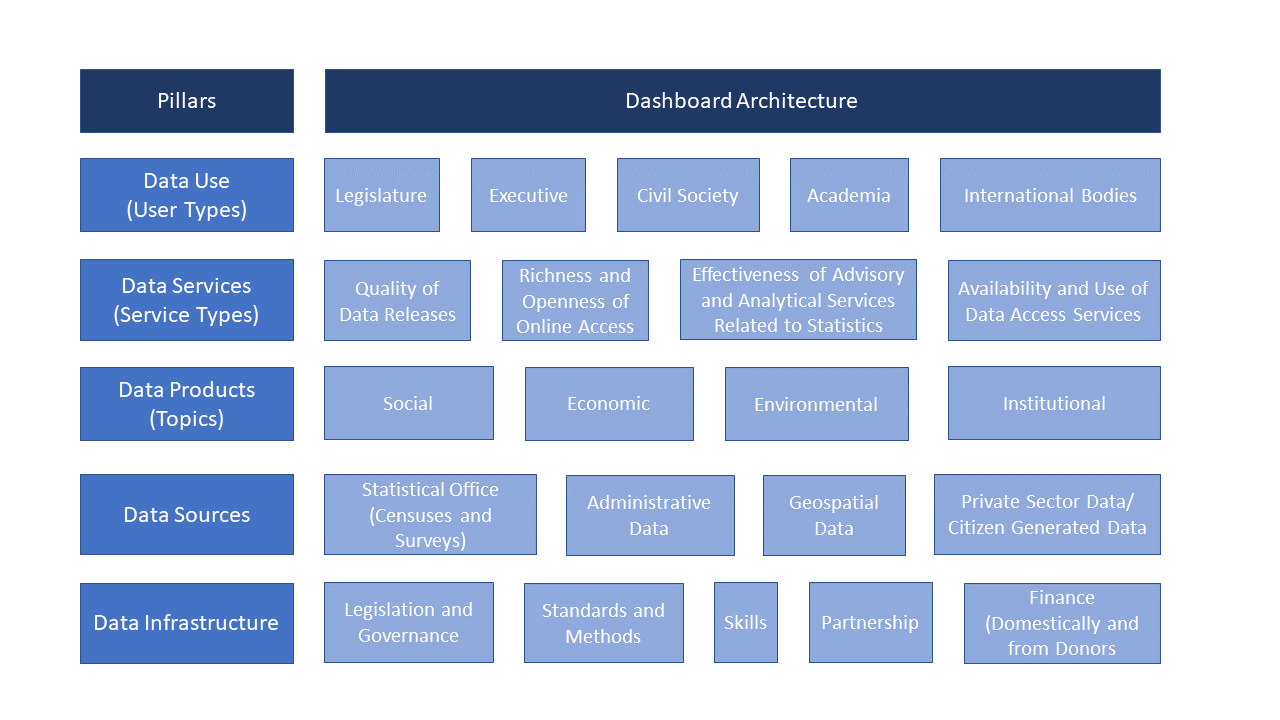
\includegraphics{SPI_dashboard.png}

Key characteristics of the SPI are: (i) uses only publicly accessible
data; (ii) transparent methodology; (iii) easily replicable; (iv)
provides a long-time series to track progress in performance; (v)
captures outcomes and supporting elements; (vi) reflects the SDGs; (vii)
facilitates at-a-glance comparisons on a global scale. We are collecting
data on indicators for the 22 components above. For dissemination, the
SPI will be presented both in the dashboard format above and as an index
for each country. Some further details on the construction of the new
SPI are provided in the Annex. These indicators should be interpreted as
a work-in-progress and are being continuously improved by the team. The
upcoming World Development Report will focus on Data for Better Lives,
and it will examine the tremendous potential of the changing data
landscape to improve the lives of poor people and consider the backdoors
that can harm people. The aim is to help bring this activity to a
conclusion in time for the World Bank World Development Report that is
due for publication in February 2021. Subsequent dissemination
activities and spin-off products (e.g., toolkits, blogs) will run into
April 2021.

\hypertarget{index-methodology}{%
\section{Index Methodology}\label{index-methodology}}

For research purposes, we create an index combining several of the
indicators together to get an overview of country performance.

The Index will contain only a subset of the dimensions from our
framework. For dimensions excluded, we either lacked a source with a
developed methodology or else the data collection for that measure was
incomplete. The sub-dimensions excluded from our index includes:

\begin{itemize}
\tightlist
\item
  Indicator 1.1: Data use by national legislature\\
\item
  Indicator 1.2: Data use by national executive branch\\
\item
  Indicator 1.3: Data use by civil society\\
\item
  Indicator 1.4: Data use by academia\\
\item
  Indicator 1.5: Data use by international organizations\\
\item
  Indicator 2.3: Advisory/ Analytical Services\\
\item
  Indicator 4.4: private/citizen generated data\\
\item
  Indicator 5.1: legislation and governance\\
\item
  Indicator 5.3: skills\\
\item
  Indicator 5.4: partnerships\\
\item
  Indicator 5.5: finance
\end{itemize}

Also the Social Protection administrative data and Labor administrative
data components are removed from the subsection on administrative data,
because of gaps in reporting of sources across countries and over time.

\includegraphics{03_index_files/figure-latex/index-2.pdf}
\includegraphics{03_index_files/figure-latex/index-3.pdf}
\includegraphics{03_index_files/figure-latex/index-4.pdf}
\includegraphics[width=9.00in,height=66.13in,keepaspectratio]{03_index_files/figure-latex/index-1.png}

\includegraphics{03_index_files/figure-latex/comparisons-1.pdf}
\includegraphics{03_index_files/figure-latex/comparisons-2.pdf}

\begin{verbatim}
## [1] 0.7368959
\end{verbatim}

\begin{verbatim}
## [1] 0.8492594
\end{verbatim}

\end{document}
